%% bare_conf.tex
%% V1.4b
%% 2015/08/26
%% by Michael Shell
%% See:
%% http://www.michaelshell.org/
%% for current contact information.
%%
%% This is a skeleton file demonstrating the use of IEEEtran.cls
%% (requires IEEEtran.cls version 1.8b or later) with an IEEE
%% conference paper.
%%
%% Support sites:
%% http://www.michaelshell.org/tex/ieeetran/
%% http://www.ctan.org/pkg/ieeetran
%% and
%% http://www.ieee.org/

%%*************************************************************************
%% Legal Notice:
%% This code is offered as-is without any warranty either expressed or
%% implied; without even the implied warranty of MERCHANTABILITY or
%% FITNESS FOR A PARTICULAR PURPOSE! 
%% User assumes all risk.
%% In no event shall the IEEE or any contributor to this code be liable for
%% any damages or losses, including, but not limited to, incidental,
%% consequential, or any other damages, resulting from the use or misuse
%% of any information contained here.
%%
%% All comments are the opinions of their respective authors and are not
%% necessarily endorsed by the IEEE.
%%
%% This work is distributed under the LaTeX Project Public License (LPPL)
%% ( http://www.latex-project.org/ ) version 1.3, and may be freely used,
%% distributed and modified. A copy of the LPPL, version 1.3, is included
%% in the base LaTeX documentation of all distributions of LaTeX released
%% 2003/12/01 or later.
%% Retain all contribution notices and credits.
%% ** Modified files should be clearly indicated as such, including  **
%% ** renaming them and changing author support contact information. **
%%*************************************************************************


% *** Authors should verify (and, if needed, correct) their LaTeX system  ***
% *** with the testflow diagnostic prior to trusting their LaTeX platform ***
% *** with production work. The IEEE's font choices and paper sizes can   ***
% *** trigger bugs that do not appear when using other class files.       ***                          ***
% The testflow support page is at:
% http://www.michaelshell.org/tex/testflow/



\documentclass[conference]{IEEEtran}
% Some Computer Society conferences also require the compsoc mode option,
% but others use the standard conference format.
%
% If IEEEtran.cls has not been installed into the LaTeX system files,
% manually specify the path to it like:
% \documentclass[conference]{../sty/IEEEtran}





% Some very useful LaTeX packages include:
% (uncomment the ones you want to load)


% *** MISC UTILITY PACKAGES ***
%
%\usepackage{ifpdf}
% Heiko Oberdiek's ifpdf.sty is very useful if you need conditional
% compilation based on whether the output is pdf or dvi.
% usage:
% \ifpdf
%   % pdf code
% \else
%   % dvi code
% \fi
% The latest version of ifpdf.sty can be obtained from:
% http://www.ctan.org/pkg/ifpdf
% Also, note that IEEEtran.cls V1.7 and later provides a builtin
% \ifCLASSINFOpdf conditional that works the same way.
% When switching from latex to pdflatex and vice-versa, the compiler may
% have to be run twice to clear warning/error messages.






% *** CITATION PACKAGES ***
%
%\usepackage{cite}
% cite.sty was written by Donald Arseneau
% V1.6 and later of IEEEtran pre-defines the format of the cite.sty package
% \cite{} output to follow that of the IEEE. Loading the cite package will
% result in citation numbers being automatically sorted and properly
% "compressed/ranged". e.g., [1], [9], [2], [7], [5], [6] without using
% cite.sty will become [1], [2], [5]--[7], [9] using cite.sty. cite.sty's
% \cite will automatically add leading space, if needed. Use cite.sty's
% noadjust option (cite.sty V3.8 and later) if you want to turn this off
% such as if a citation ever needs to be enclosed in parenthesis.
% cite.sty is already installed on most LaTeX systems. Be sure and use
% version 5.0 (2009-03-20) and later if using hyperref.sty.
% The latest version can be obtained at:
% http://www.ctan.org/pkg/cite
% The documentation is contained in the cite.sty file itself.






% *** GRAPHICS RELATED PACKAGES ***
%
\usepackage{graphicx}
\DeclareGraphicsExtensions{.pdf,.png,.jpg}

\ifCLASSINFOpdf
  % \usepackage[pdftex]{graphicx}
  % declare the path(s) where your graphic files are
  % \graphicspath{{../pdf/}{../jpeg/}}
  % and their extensions so you won't have to specify these with
  % every instance of \includegraphics
  % \DeclareGraphicsExtensions{.pdf,.jpeg,.png}
\else
  % or other class option (dvipsone, dvipdf, if not using dvips). graphicx
  % will default to the driver specified in the system graphics.cfg if no
  % driver is specified.
  %\usepackage[dvips]{graphicx}
  % declare the path(s) where your graphic files are
  %\graphicspath{{eps}}
  % and their extensions so you won't have to specify these with
  % every instance of \includegraphics
  % \DeclareGraphicsExtensions{.eps}
\fi
% graphicx was written by David Carlisle and Sebastian Rahtz. It is
% required if you want graphics, photos, etc. graphicx.sty is already
% installed on most LaTeX systems. The latest version and documentation
% can be obtained at: 
% http://www.ctan.org/pkg/graphicx
% Another good source of documentation is "Using Imported Graphics in
% LaTeX2e" by Keith Reckdahl which can be found at:
% http://www.ctan.org/pkg/epslatex
%
% latex, and pdflatex in dvi mode, support graphics in encapsulated
% postscript (.eps) format. pdflatex in pdf mode supports graphics
% in .pdf, .jpeg, .png and .mps (metapost) formats. Users should ensure
% that all non-photo figures use a vector format (.eps, .pdf, .mps) and
% not a bitmapped formats (.jpeg, .png). The IEEE frowns on bitmapped formats
% which can result in "jaggedy"/blurry rendering of lines and letters as
% well as large increases in file sizes.
%
% You can find documentation about the pdfTeX application at:
% http://www.tug.org/applications/pdftex





% *** MATH PACKAGES ***
%
%\usepackage{amsmath}
% A popular package from the American Mathematical Society that provides
% many useful and powerful commands for dealing with mathematics.
%
% Note that the amsmath package sets \interdisplaylinepenalty to 10000
% thus preventing page breaks from occurring within multiline equations. Use:
%\interdisplaylinepenalty=2500
% after loading amsmath to restore such page breaks as IEEEtran.cls normally
% does. amsmath.sty is already installed on most LaTeX systems. The latest
% version and documentation can be obtained at:
% http://www.ctan.org/pkg/amsmath





% *** SPECIALIZED LIST PACKAGES ***
%
%\usepackage{algorithmic}
% algorithmic.sty was written by Peter Williams and Rogerio Brito.
% This package provides an algorithmic environment fo describing algorithms.
% You can use the algorithmic environment in-text or within a figure
% environment to provide for a floating algorithm. Do NOT use the algorithm
% floating environment provided by algorithm.sty (by the same authors) or
% algorithm2e.sty (by Christophe Fiorio) as the IEEE does not use dedicated
% algorithm float types and packages that provide these will not provide
% correct IEEE style captions. The latest version and documentation of
% algorithmic.sty can be obtained at:
% http://www.ctan.org/pkg/algorithms
% Also of interest may be the (relatively newer and more customizable)
% algorithmicx.sty package by Szasz Janos:
% http://www.ctan.org/pkg/algorithmicx




% *** ALIGNMENT PACKAGES ***
%
\usepackage{array}
% Frank Mittelbach's and David Carlisle's array.sty patches and improves
% the standard LaTeX2e array and tabular environments to provide better
% appearance and additional user controls. As the default LaTeX2e table
% generation code is lacking to the point of almost being broken with
% respect to the quality of the end results, all users are strongly
% advised to use an enhanced (at the very least that provided by array.sty)
% set of table tools. array.sty is already installed on most systems. The
% latest version and documentation can be obtained at:
% http://www.ctan.org/pkg/array


% IEEEtran contains the IEEEeqnarray family of commands that can be used to
% generate multiline equations as well as matrices, tables, etc., of high
% quality.




% *** SUBFIGURE PACKAGES ***
%\ifCLASSOPTIONcompsoc
%  \usepackage[caption=false,font=normalsize,labelfont=sf,textfont=sf]{subfig}
%\else
%  \usepackage[caption=false,font=footnotesize]{subfig}
%\fi
% subfig.sty, written by Steven Douglas Cochran, is the modern replacement
% for subfigure.sty, the latter of which is no longer maintained and is
% incompatible with some LaTeX packages including fixltx2e. However,
% subfig.sty requires and automatically loads Axel Sommerfeldt's caption.sty
% which will override IEEEtran.cls' handling of captions and this will result
% in non-IEEE style figure/table captions. To prevent this problem, be sure
% and invoke subfig.sty's "caption=false" package option (available since
% subfig.sty version 1.3, 2005/06/28) as this is will preserve IEEEtran.cls
% handling of captions.
% Note that the Computer Society format requires a larger sans serif font
% than the serif footnote size font used in traditional IEEE formatting
% and thus the need to invoke different subfig.sty package options depending
% on whether compsoc mode has been enabled.
%
% The latest version and documentation of subfig.sty can be obtained at:
% http://www.ctan.org/pkg/subfig




% *** FLOAT PACKAGES ***
%
%\usepackage{fixltx2e}
% fixltx2e, the successor to the earlier fix2col.sty, was written by
% Frank Mittelbach and David Carlisle. This package corrects a few problems
% in the LaTeX2e kernel, the most notable of which is that in current
% LaTeX2e releases, the ordering of single and double column floats is not
% guaranteed to be preserved. Thus, an unpatched LaTeX2e can allow a
% single column figure to be placed prior to an earlier double column
% figure.
% Be aware that LaTeX2e kernels dated 2015 and later have fixltx2e.sty's
% corrections already built into the system in which case a warning will
% be issued if an attempt is made to load fixltx2e.sty as it is no longer
% needed.
% The latest version and documentation can be found at:
% http://www.ctan.org/pkg/fixltx2e


%\usepackage{stfloats}
% stfloats.sty was written by Sigitas Tolusis. This package gives LaTeX2e
% the ability to do double column floats at the bottom of the page as well
% as the top. (e.g., "\begin{figure*}[!b]" is not normally possible in
% LaTeX2e). It also provides a command:
%\fnbelowfloat
% to enable the placement of footnotes below bottom floats (the standard
% LaTeX2e kernel puts them above bottom floats). This is an invasive package
% which rewrites many portions of the LaTeX2e float routines. It may not work
% with other packages that modify the LaTeX2e float routines. The latest
% version and documentation can be obtained at:
% http://www.ctan.org/pkg/stfloats
% Do not use the stfloats baselinefloat ability as the IEEE does not allow
% \baselineskip to stretch. Authors submitting work to the IEEE should note
% that the IEEE rarely uses double column equations and that authors should try
% to avoid such use. Do not be tempted to use the cuted.sty or midfloat.sty
% packages (also by Sigitas Tolusis) as the IEEE does not format its papers in
% such ways.
% Do not attempt to use stfloats with fixltx2e as they are incompatible.
% Instead, use Morten Hogholm'a dblfloatfix which combines the features
% of both fixltx2e and stfloats:
%
% \usepackage{dblfloatfix}
% The latest version can be found at:
% http://www.ctan.org/pkg/dblfloatfix




% *** PDF, URL AND HYPERLINK PACKAGES ***
%
%\usepackage{url}
% url.sty was written by Donald Arseneau. It provides better support for
% handling and breaking URLs. url.sty is already installed on most LaTeX
% systems. The latest version and documentation can be obtained at:
% http://www.ctan.org/pkg/url
% Basically, \url{my_url_here}.




% *** Do not adjust lengths that control margins, column widths, etc. ***
% *** Do not use packages that alter fonts (such as pslatex).         ***
% There should be no need to do such things with IEEEtran.cls V1.6 and later.
% (Unless specifically asked to do so by the journal or conference you plan
% to submit to, of course. )


% correct bad hyphenation here
\hyphenation{op-tical net-works semi-conduc-tor}


\begin{document}
%
% paper title
% Titles are generally capitalized except for words such as a, an, and, as,
% at, but, by, for, in, nor, of, on, or, the, to and up, which are usually
% not capitalized unless they are the first or last word of the title.
% Linebreaks \\ can be used within to get better formatting as desired.
% Do not put math or special symbols in the title.
\title{Smart Shoebox\\ (Shoes care solution utilizing IoT concept)}


% author names and affiliations
% use a multiple column layout for up to three different
% affiliations
\author{\IEEEauthorblockN{Ko Byunghee, Kwon Gyuhyeok, Kim Junghyun, Shin Minki}
\IEEEauthorblockA{Information System Department\\College of Engineering\\
Hanyang University\\
Seoul, South Korea}}

% conference papers do not typically use \thanks and this command
% is locked out in conference mode. If really needed, such as for
% the acknowledgment of grants, issue a \IEEEoverridecommandlockouts
% after \documentclass

% for over three affiliations, or if they all won't fit within the width
% of the page, use this alternative format:
% 
%\author{\IEEEauthorblockN{Michael Shell\IEEEauthorrefmark{1},
%Homer Simpson\IEEEauthorrefmark{2},
%James Kirk\IEEEauthorrefmark{3}, 
%Montgomery Scott\IEEEauthorrefmark{3} and
%Eldon Tyrell\IEEEauthorrefmark{4}}
%\IEEEauthorblockA{\IEEEauthorrefmark{1}School of Electrical and Computer Engineering\\
%Georgia Institute of Technology,
%Atlanta, Georgia 30332--0250\\ Email: see http://www.michaelshell.org/contact.html}
%\IEEEauthorblockA{\IEEEauthorrefmark{2}Twentieth Century Fox, Springfield, USA\\
%Email: homer@thesimpsons.com}
%\IEEEauthorblockA{\IEEEauthorrefmark{3}Starfleet Academy, San Francisco, California 96678-2391\\
%Telephone: (800) 555--1212, Fax: (888) 555--1212}
%\IEEEauthorblockA{\IEEEauthorrefmark{4}Tyrell Inc., 123 Replicant Street, Los Angeles, California 90210--4321}}




% use for special paper notices
%\IEEEspecialpapernotice{(Invited Paper)}




% make the title area
\maketitle

% As a general rule, do not put math, special symbols or citations
% in the abstract
\begin{abstract}
This document is about the realization of automatic remote control for shoesthrough IoT. We will make smart shoes cabinet that provides this kind of features with other different kind of functions.
\\
\end{abstract}

\begin{IEEEkeywords}
shoebox; shoes care; shoes rack; IoT;
\end{IEEEkeywords}




% no keywords




% For peer review papers, you can put extra information on the cover
% page as needed:
% \ifCLASSOPTIONpeerreview
% \begin{center} \bfseries EDICS Category: 3-BBND \end{center}
 %\fi
%
% For peerreview papers, this IEEEtran command inserts a page break and
% creates the second title. It will be ignored for other modes.

\IEEEpeerreviewmaketitle

%TABLE1
\begin{table}[!t]
\renewcommand{\arrayrulewidth}{1pt}
\renewcommand{\arraystretch}{2.5}
\begin{tabular}
{|m{1.7cm}|m{1.7cm}|p{.47\linewidth}|}\hline

Role & Name & Task and description etc\\ \hline
User & Kwon Gyuhyeok & Suggest the actual features for the Smart Shoebox users can feel comfortable and interesting to use\\ \hline
Customer & Shin Minki & Suggest the actual features for the Smart Shoebox customers can feel comfortable and interesting to use\\ \hline
Software developer & Kim Junghyun & Focusing on the Technical aspects of the Smart Shoebox while developing \\ \hline
Development manager & Ko Byunghee & Consider the service side of the Smart Shoebox while developing the system\\ \hline

\end{tabular}
\\
\\
\caption{Role Assignment}
\label{tab:template}
\end{table}



% 1. introduction
\section{Introduction}
% no \IEEEPARstart
Many people experience difficulty managing their own shoes in a decent and pleasant form. Especially for the people living alone, keeping shoes clean and sweet smelling becomes a tough task to manage. When it rains, shoes get wet and dirty. Can you imagine the smell and feel of the shoe? Even worse the smell starts from the entrance to the place where you will go to sleep. This is when the actual management features are required.

What if someone or something could take care of my shoes periodically and automatically. If the shoes could be managed regularly with the aspects of humidity, temperature, and sterilization, it will save money and also provide a pleasant day with a cozy footwear. To realize the concepts of taking care of our shoes, we will develop a shoebox which manages shoes condition by controlling humidity and temperature automatically and periodically. 

We are going to use Arduino to support with humidity and temperature recognition by receiving inputs through switches or sensors. Internet of Things (IoT) is also on the base of the idea. The ability to control things (especially shoes in this case) through internet is the main concept we are trying to realize. We are looking forward to create an integrated service tool such as situation awareness, automatic computing, self-growing. \\
% You must have at least 2 lines in the paragraph with the drop letter
% (should never be an issue)


% 2. requirement
\section{Requirement}

\subsection{Optimizing environment function}
When we wear shoes, they easily become in a state of high temperature and humidity which causes the disgusting smell, which is also the best environment for bacteria to grow. As a result, there is a need to control the condition of the cabinet keeping the shoes. To provide an optimized environment automatically and also on user?s demand is the goal. (There is a need for defining optimized temperature and humidity)
\subsubsection{Temperature/Humidity control through electric fan (automatic)}
The sensor receives temperature and humidity as inputs and provides an optimized environment as an output.
\subsubsection{Temperature/Humidity control through ultraviolet lamp (automatic)}
The sensor receives temperature and humidity as inputs and provides an optimized temperature and humidity as output.
\subsubsection{Drying feature (on demand)}
In case the user's shoes get wet by rain or other liquids the user can request for drying will operate (1), (2).
\subsubsection{Sterilization function (on demand)}
In case the user feels the need for sterilization, user can request for this function, which operates (1), (2).
This function (4) differs from (3) in degrees of intensity.
\subsubsection{Deodorization function (on demand)}
In case the user feels the need for deodorization, user can request for this function, which triggers a deodorant to shoot out.
\subsubsection{Deodorization function (automatic)}
The user can set regular intervals to trigger the deodorant to shoot out.
\subsubsection{Intensity control feature}
The user can choose the intensity level of (1), (2). Intensity is calculated as number between 1 to 5.\\


\subsection{Management function}
Different type of shoes requires different type of proper cares. The shoe rack needs to understand and recognize the shoes type and provide a proper management for the shoes.
(Modeling : changing ambiguous information into actual concept.)
\subsubsection{Shoe categorization function (bar-code scanning)}
Shoe categorization through capturing the barcode for the shoes.
\subsubsection{Shoe categorization function (user input based)}
Shoe categorization through selected category of the user.
\subsubsection{Shoe categorization function (captured image)}
Shoe categorization through captured images of the shoes.
\subsubsection{Shoe categorization function (3D scanning)}
Shoe categorization through 3D scanning of the shoes.
\subsubsection{Setting the proper management tool}
After Shoe categorization, based on the shoes category, the shoe rack provides the proper setting.
(There is a need for defining proper setting for each category)
The proper setting is different in the aspect of the intensity from Optimization environment function.\\


\subsection{Analysis function}
To keep the user's shoes in high quality we can provide an analysis for the shoes the user own.
\subsubsection{Absence of shoes analysis (Base information)}
We have decided to analyze the absence of shoes by sensor and use it as a base information for other analysis functions.
\subsubsection{Durability analysis}
Durability is set to decrease by the time the shoe has been put on increases. 
\subsubsection{Life prediction analysis}
Based on the information of (1), we provide the expected  life of the shoes.
\subsubsection{Preference analysis (personal)}
Based on the information of (1) for one user, we provide the preference information of the shoes. More the user put on, more the preference increases.
\subsubsection{Preference analysis (general)}
Based on the information of (1) for a number of users, we provide the preference information of the shoes for general aspect. Using this Big data, the user can know which shoes are popular nowadays.
\subsubsection{Frequency analysis}
Based on the information of (1), we provide the frequency information for the shoes.\subsubsection{Walking habit analysis (health care)}
Based on the information flatness of the shoes , we provide the information about walking habit of the users.\\


\subsection{Recommendation function}
Smart Shoes cabinet will provide recommendation information with percentages based on different kind of aspects. Of course the final choice is up to the user.
\subsubsection{Recommendation based on weather forecast }
With weather API, the proper type of shoes is recommended.
\subsubsection{ Recommendation based on the use of shoes}
Recommending the shoes type which matches with the user?s activity.
\subsubsection{Recommendation based on the color of shoes}
Recommending the shoes color which balances with the users clothing color.
\subsubsection{ Notice of recommendation rate by color}
Showing the recommendation rate by different colors. For example, if the shoes are recommended, a specific color will appear on the shoe rack or on the screen the user is looking at. 
\subsubsection{Notice of recommendation rate by percentage}
Showing the recommendation rate by percentage. If the shoes are recommended strongly, the percentage will appear on the shoe rack or on the screen the user is looking at. \\


\subsection{Notification function}
Shoes easily get dirty, since when people do activities, shoes are the first thing that touches the ground. The shoes cabinet will provide notification for contamination of dirt or rainwater by checking on the weight difference.
\subsubsection{Recognition of contamination by sensor}
With the increased weight, notification is given for contamination.
\subsubsection{Notification for contamination by message}
After the recognition of contamination, the information is notified to the user through messages.\\


\subsection{Networking / Remote control function (UI)}
Without the function for internet control, it becomes nothing more than a drying machine. With this networking function on the base, the user is able to take care of the users shoes any time, anywhere. This is the most important feature we will concentrate on. Providing the IoT environment is the main goal. 
\subsubsection{Control function through web programming (main)}
With web based program, the user can interact with the smart shoe care software and other provided information.
\subsubsection{Control function through mobile (sub)}
With mobile application, the user can interact with the smart shoe care software and other provided information.
\subsubsection{Control function through embedded system (sub)}
With embedded system, the user can interact with the smart shoe care software and other provided information.\\

% 3. development environment
\section{Development Environment}

\subsection{Choice of software development platform}
\subsubsection{Platform used for developing}package
 We will use both Windows and MAC OS . Since Windows is the most popular OS used worldwide and MAC OS is the second most popular OS leaving out all the other versions of Windows. We thought MAC OS X will become more popular. We also thought using other OS besides windows will mean a lot for us to use another environment to develop a software.
 %image1
\begin{figure}[htbp]
\begin{center}
    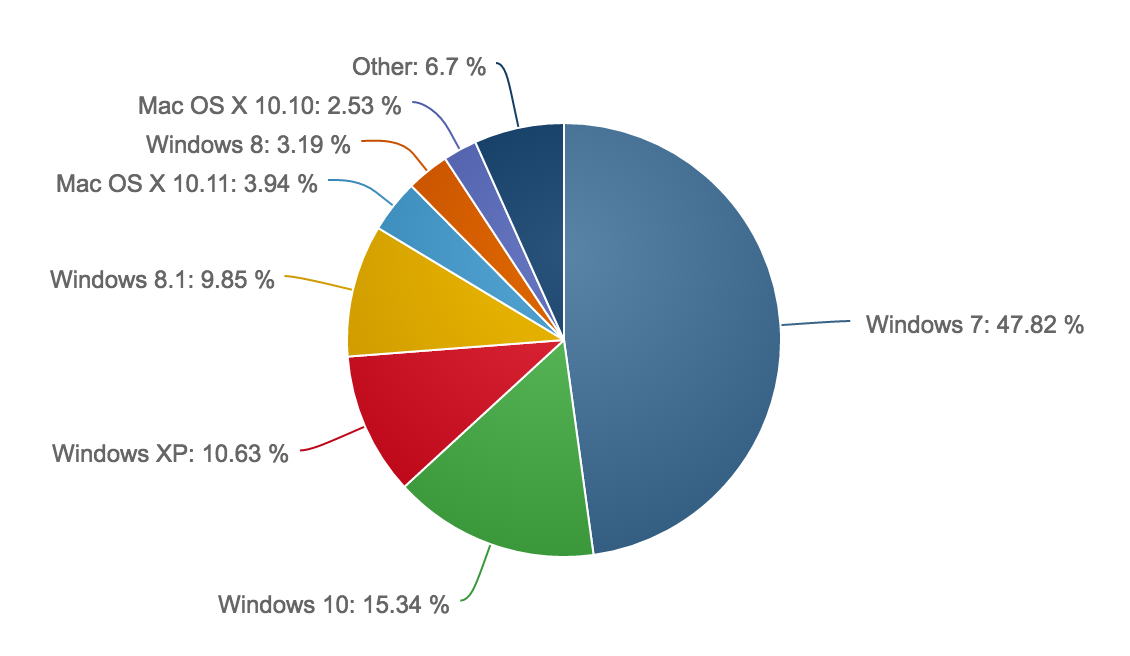
\includegraphics[scale=0.45]{marketshare}
    \caption{Market share reports (January, 2016 to March, 2016)} \label{fig:label}
\end{center}
\end{figure}

\subsubsection{Programming language used for developing}
We are using Arduino, mySQL, Ruby and HTML. We are trying to provide a web service with arduino acting inside the Smart Shoebox. The frontend will be using html and css, while the backend will be using ruby and ruby on rails as a application framework. If we think of the server as a localhost, we might be using only ruby and ruby on rails for the server without MySQL.

%TABLE2
\begin{table}
\renewcommand{\arrayrulewidth}{1pt}
\renewcommand{\arraystretch}{2.5}
\begin{tabular}
{|p{3.5cm}|p{.5\linewidth}|}\hline

Programming language & Reason\\ \hline
Arduino(hardware) &The main hardware part of our project is based on Arduino. The Smart Shoebox has functions to work provide behavioral motions such as recognizing the temperature and humidity of the shoebox, turning on the fan or infrared lamp as a result of it and so on.
 \\ \hline
MySQL(server side) & We need to have a database to save information about the shoes, users. To easily get and set and manage the information, we have decided to use a database management tool. \\ \hline
Ruby & We first thought of php for the work between the server and web side environment, since we have all learned php in another course. Though we thought it would be much better to learn a new language for this project. Ruby on rails was the interesting programming language in the aspect that it shortens and simplifies the code much more than the php. \\ \hline
HTML5 and CSS3(client side) & We have decided the user interface environment as a web-based structure. The functions of Smart Shoebox will be triggered and managed in the web. \\ \hline

\end{tabular}
\\
\\
\caption{Programming language used for developing}
\label{tab:template}
\end{table}


\subsubsection{Cost estimation (Software / Hardware)}
TABLE III and TABLE IV
\\
\\
%TABLE3
\begin{table}
\renewcommand{\arrayrulewidth}{1pt}
\renewcommand{\arraystretch}{2}
\begin{tabular}
{|p{4cm}|p{.5\linewidth}|}\hline

Device & Price (won)\\ \hline
Arduino uno R3 & 7,500\\ \hline
Bread board & 2,400\\ \hline
Wifi module(ESP8266) & 9,000\\ \hline
Temperature Humidity sensor & 3,000\\ \hline
Pressure Sensor & 14,000\\ \hline
Fan(actuator) & 4,000\\ \hline
Board & 2,000\\ \hline
USB cable & 500\\ \hline
jump wire & 2,500\\ \hline
M-F wire & 2,000\\ \hline
Resistance & 200(5 per unit)\\ \hline
Small LED lamp & 1,000\\ \hline
AA battery & 1,200\\ \hline
transistor & 500 \\ \hline
TOTAL & 49,800 \\ \hline

\end{tabular}
\\
\\
\caption{Cost estimation(Hardware)}
\label{tab:template}
\end{table}

%TABLE4
\begin{table}
\renewcommand{\arrayrulewidth}{1pt}
\renewcommand{\arraystretch}{2}
\begin{tabular}
{|p{4cm}|p{.5\linewidth}|}\hline

Software&Task Description\\ \hline
Source Tree(v1.8.3)&Version control \\ \hline
Git(v2.8.1)&Project control\\ \hline
Github&Remote repository\\ \hline
Sublime Text3(3103)&Text editor\\ \hline
mockflow&Wireframe creation\\ \hline
Mac OS X El Capitan&Operating System\\ \hline
Windows 8 / 10&Operating System\\ \hline
Arduino(v1.6.8)&Text editor for Arduino\\ \hline
TOTAL & 0 \\ \hline


\end{tabular}
\\
\\
\caption{Cost estimation(software)}
\label{tab:template}
\end{table}


\subsection{Software in use}
We have researched to find out if there is any existing software or algorithm in use doing a similar task we are trying to provide. We were really surprised to find so much information related to our project. There was a lot of algorithms and systems during the research. The most interesting and related ones were the three below.
\subsubsection{Temperature Humidity Control system}
As anyone can think of the air conditioner or greenhouse there were already a lot of systems and devices doing the actual part of our project to control the temperature and humidity for the given environment. (For our home, or for growing plants in the optimized temperature and humidity, and so on.) Even there were a lot of information about making the Arduino actually work as we planned to.
 %image2
\begin{figure}[htbp]
\begin{center}
    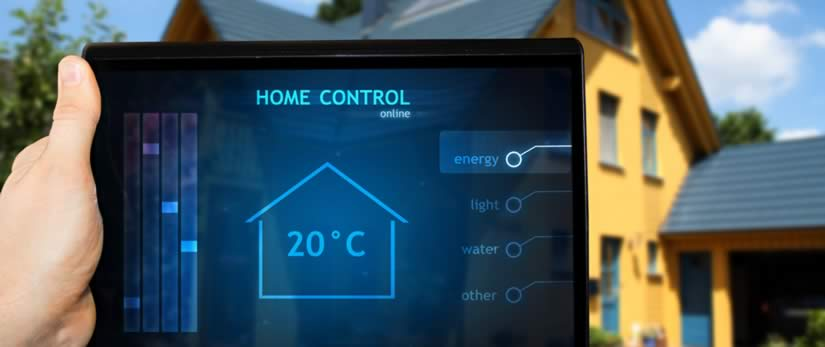
\includegraphics[scale=1.2]{temperature_control}
    \caption{Advance Temperature Control (http://infusionva.com/)} \label{fig:label}
\end{center}
\end{figure}

%image3
\begin{figure}[htbp]
\begin{center}
    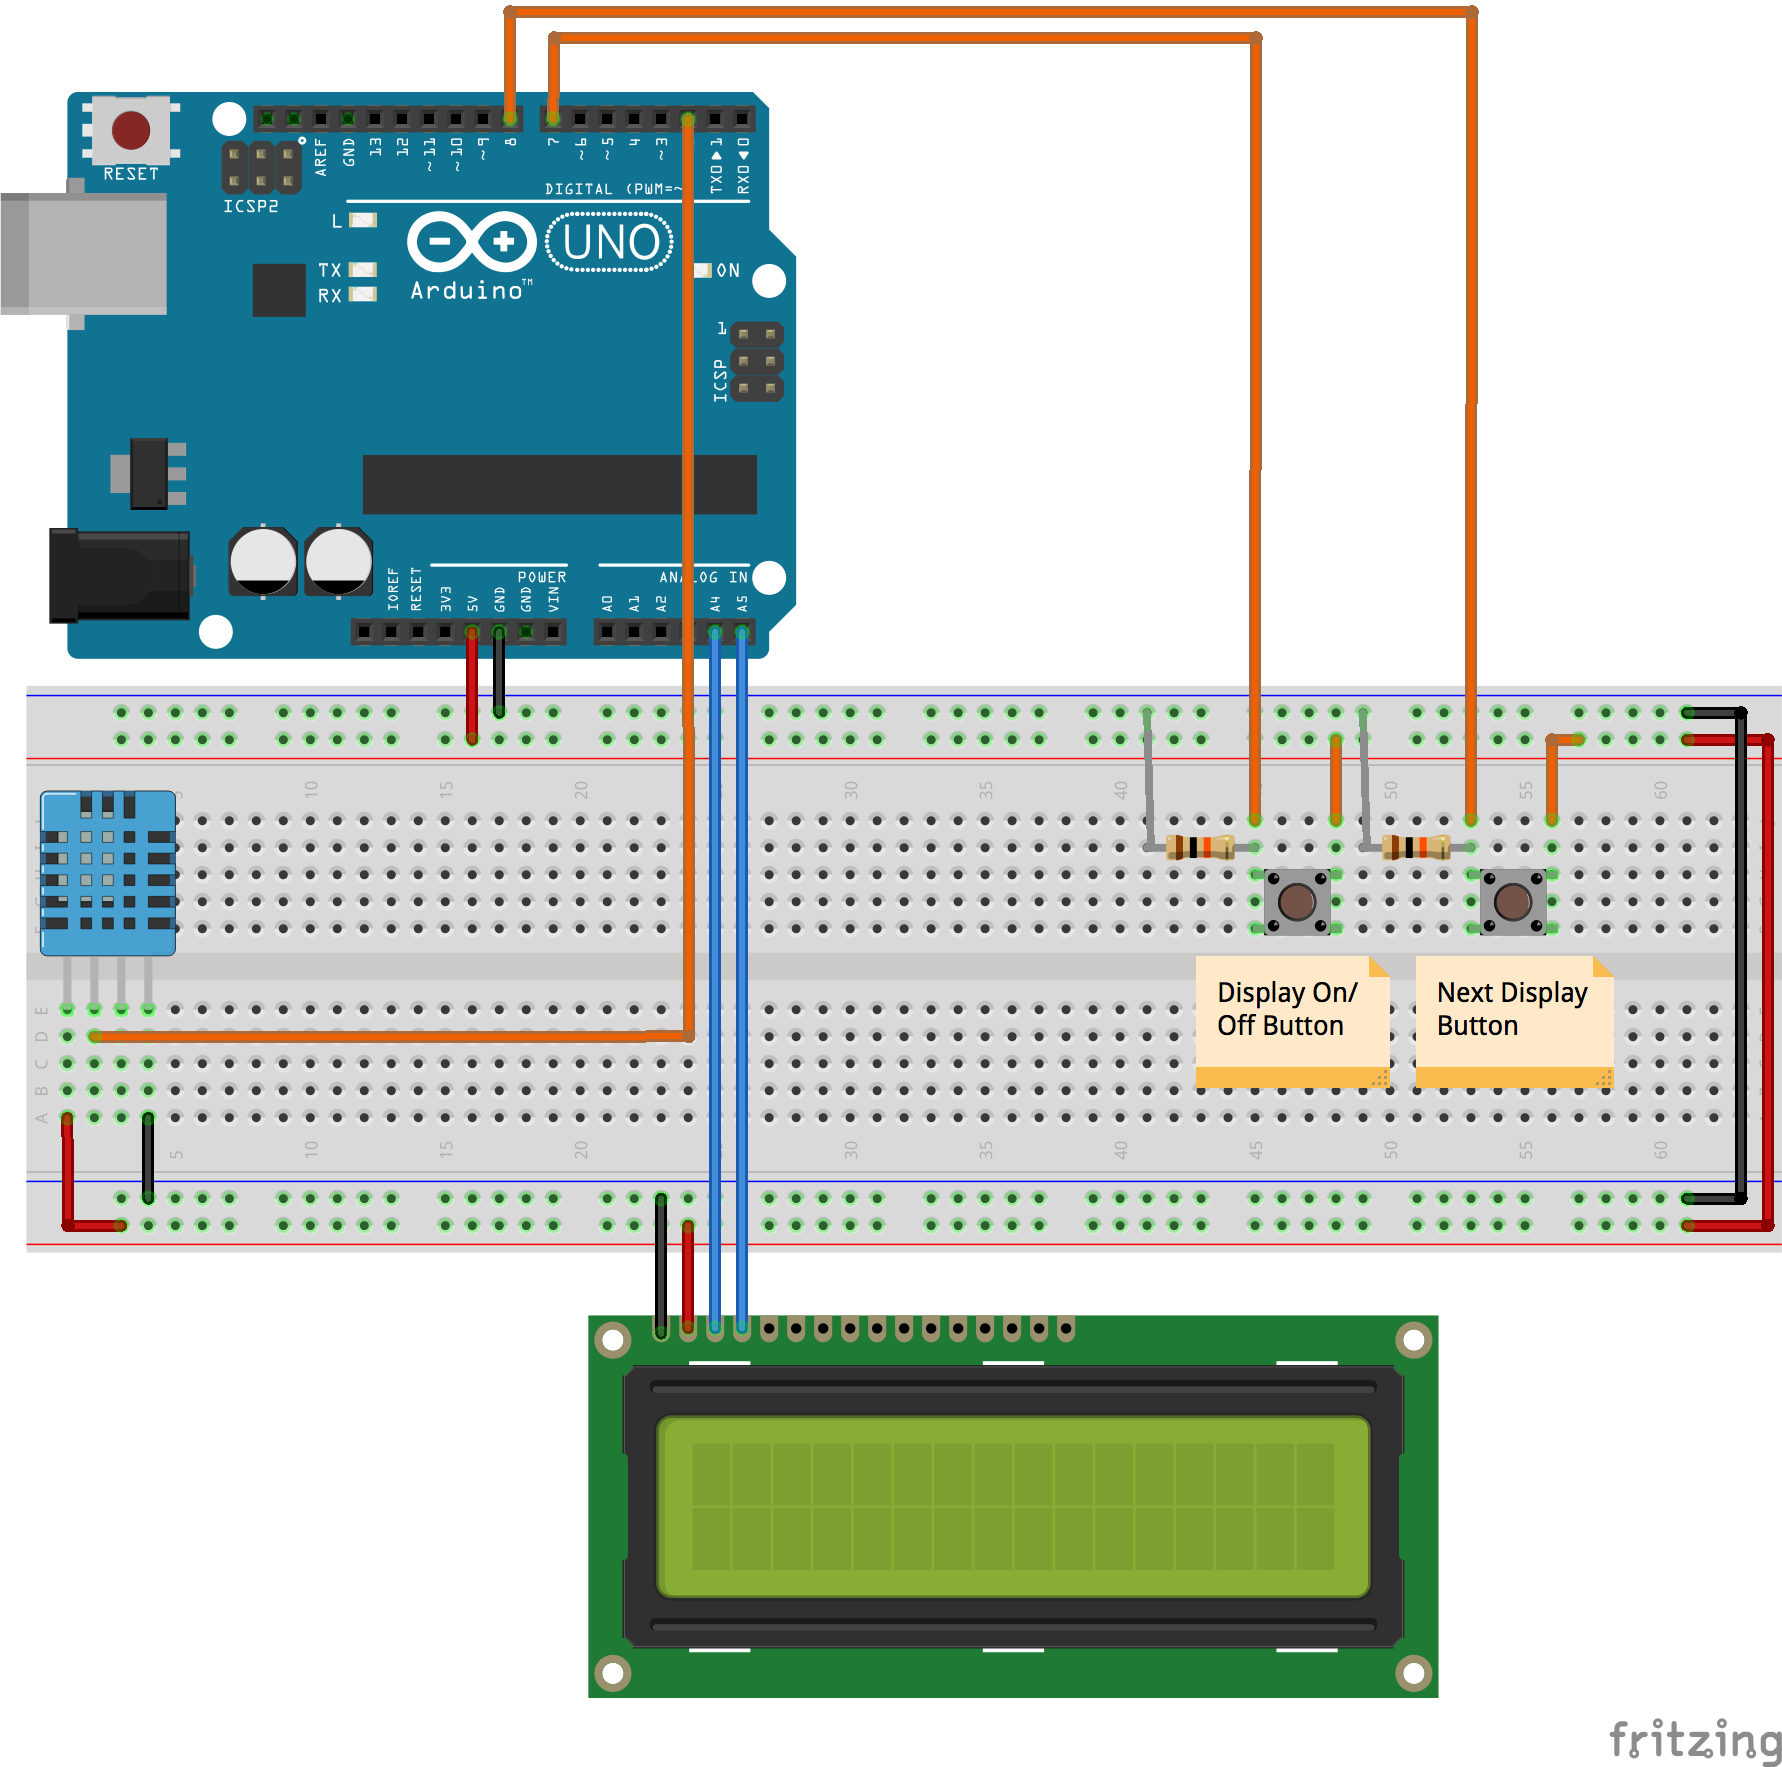
\includegraphics[scale=0.4]{arduino}
    \caption{Airconditioner automatic control through Arduino} \label{fig:label}
\end{center}
\end{figure}


\subsubsection{Recommendation System }
There is an extensive class of Web applications that involve predicting user responses to options. Such a facility is called a recommendation system.
 In Figure above we see an example utility matrix, representing users? ratings of movies on a 1?5 scale, with 5 the highest rating. Blanks represent the situation where the user has not rated the movie. The movie names are HP1, HP2, and HP3 for Harry Potter I, II, and III, TW for Twilight, and SW1, SW2, and SW3 for Star Wars episodes 1, 2, and 3. The users are represented by capital letters A through D.
 The goal of a recommendation system is to predict the blanks in the utility matrix. 
This recommendation system was in common with our project in the point that we will provide a recommendation information for the shoes with the weather APT and color of the shoes matching with the user?s clothes.
%image4
\begin{figure}[htbp]
\begin{center}
    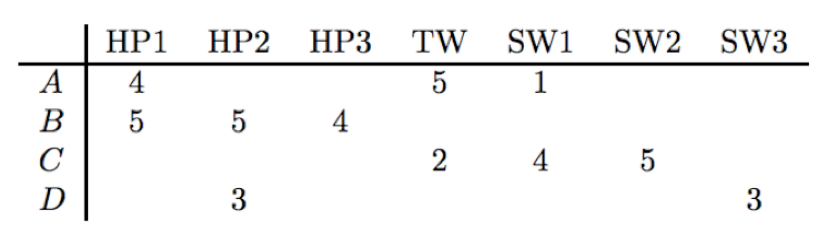
\includegraphics[scale=0.5]{utilitymatrix}
    \caption{utilitymatrix} \label{fig:label}
\end{center}
\end{figure}

\subsubsection{Classification Algorithm in datamining}
Basic Principle (Inductive Learning Hypothesis): Any hypothesis found to approximate the target function well over a sufficiently large set of training examples will also approximate the target function well over other unobserved examples.
%image5
\begin{figure}[htbp]
\begin{center}
    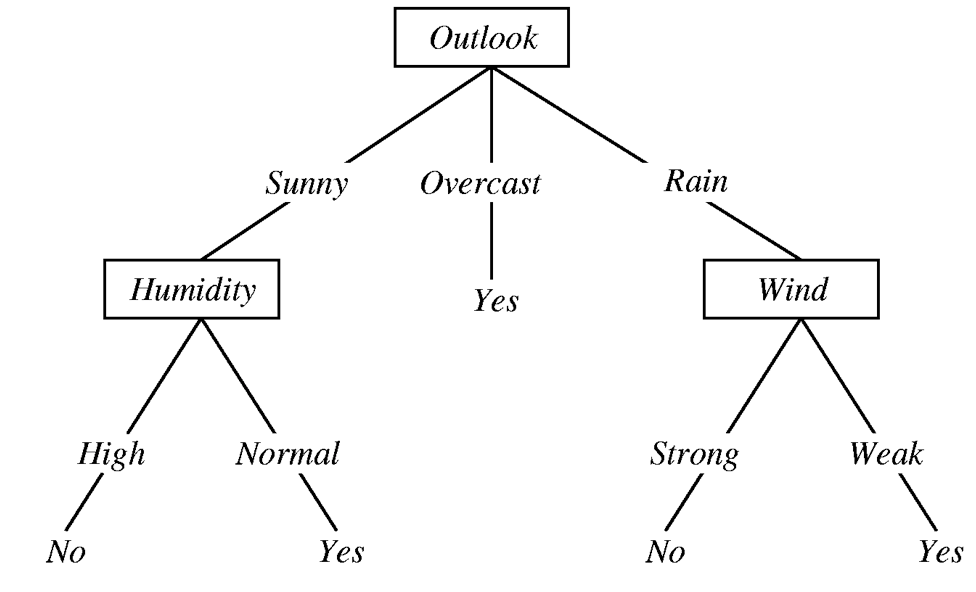
\includegraphics[scale=0.5]{decisiontree_learning}
    \caption{decisiontree learning} \label{fig:label}
\end{center}
\end{figure}

This algorithm was in common with our project in the point that we will classify the shoes. 


\subsection{Task Distribution}
We have decided to distribute the project in big parts to make each participants to be responsible for the assigned parts. Still every person has to know how the project is going on in a big picture while being responsible for the assigned part.
%TABLE5
\begin{table}[!t]
\renewcommand{\arrayrulewidth}{1pt}
\renewcommand{\arraystretch}{2.5}
\begin{tabular}
{|p{4cm}|p{4cm}|}\hline
Name & Responsible Part\\ \hline
Kwon GyuHyeok&Arduino\\ \hline
Shin MinKi&MySQL\\ \hline
Kim JungHyun&Wireless fidelity control\\ \hline
Ko ByungHee&Ruby on rails\\ \hline
\end{tabular}
\\
\\
\caption{Task Distribution}
\label{tab:template}
\end{table}
\\
\\
\\
\\
\\
\\
\\

% 4. specification
\section{Specification}
The specification is mostly in pseudocode and additionally graphs and charts will be used to specify the requirements. Particularly, mockflow will be used to wireframe the user interface. The pseudocode is a little bit close to the programming languages we have already learned during other courses while disregarding the details of the grammar.
\subsection{Optimizing environment function}
\subsubsection{Temperature/Humidity control through electric fan (automatic)}
\subsubsection{Temperature/Humidity control through ultraviolet lamp (automatic)}
The arduino sensor receives temperature and humidity as inputs and truns on fan and ultraviolet lamp when temperature drops below 15 Celsius degree or humidity is higher than 
%image
\begin{figure}[htbp]
\begin{center}
    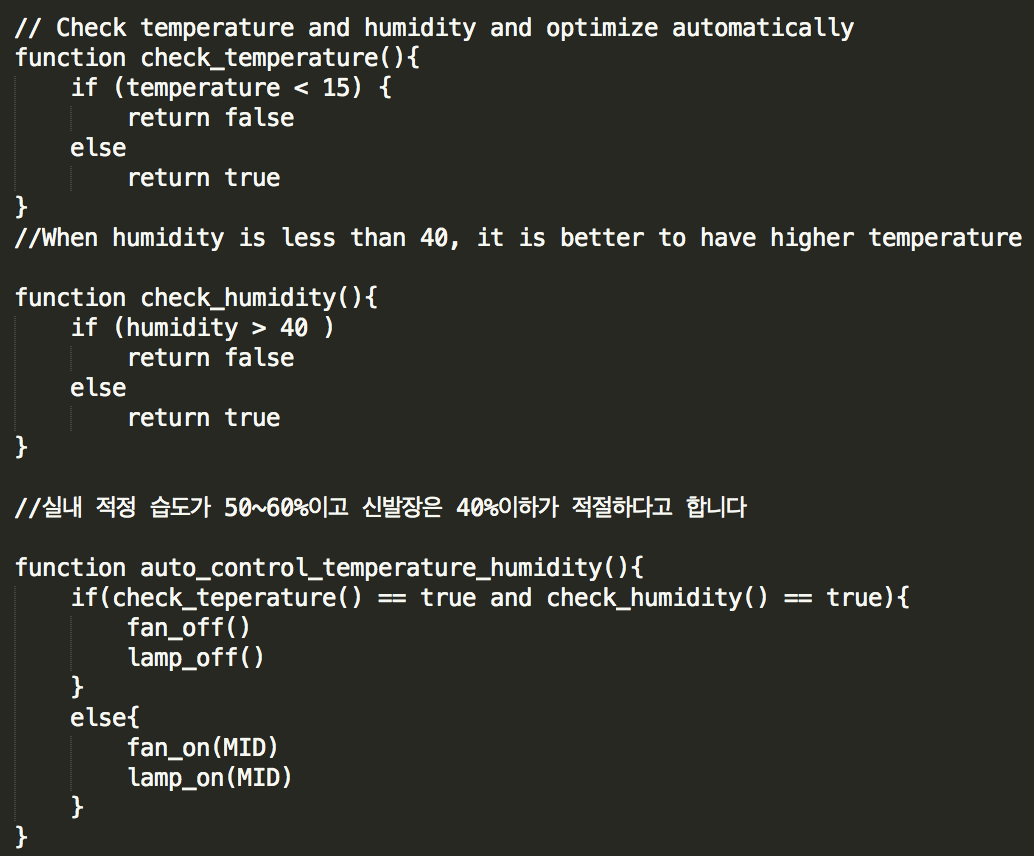
\includegraphics[scale=0.48]{optimization1}
    \label{fig:label}
\end{center}
\end{figure}
\subsubsection{Drying feature (on demand)}
In case the user?s shoes get wet by rain or other liquids the user can request for drying function. The function will turn on fan on maximum rate and intensity of lamp will be middle.
%image
\begin{figure}[htbp]
\begin{center}
    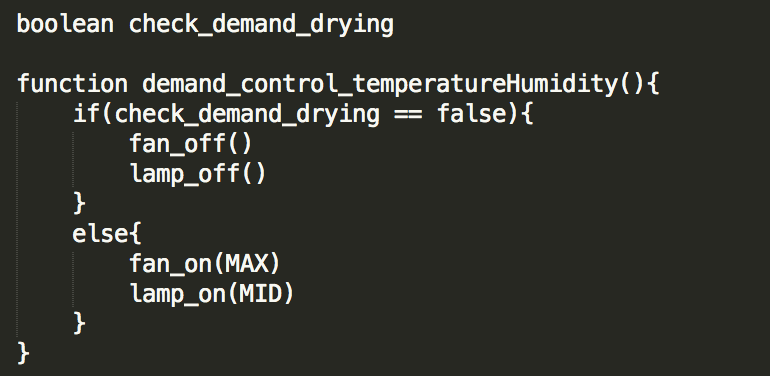
\includegraphics[scale=0.6]{optimization2}
    \label{fig:label}
\end{center}
\end{figure}
\subsubsection{Sterilization function (on demand)}
In case the user feels the need for sterilization, user can request for this function. The function will turn on fan on middle rate and intensity of lamp will be maximum.
%image
\begin{figure}[htbp]
\begin{center}
    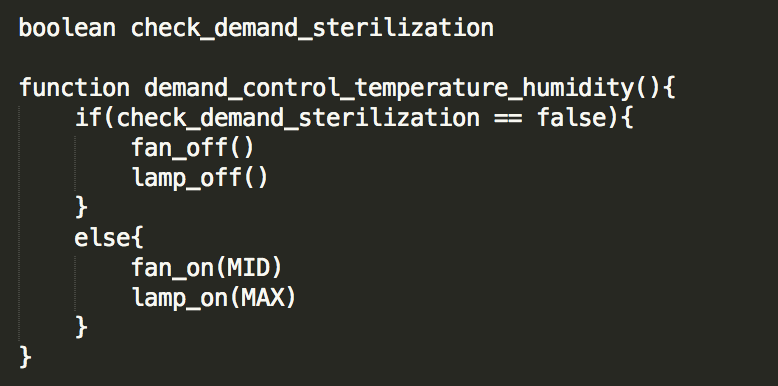
\includegraphics[scale=0.6]{optimization3}
    \label{fig:label}
\end{center}
\end{figure}
\subsubsection{Deodorization function (on demand)}
In case the user feels the need for deodorization, user can request for this function, which triggers a deodorant to shoot out. The Arduino will trigger the deodorant.
%image
\begin{figure}[htbp]
\begin{center}
    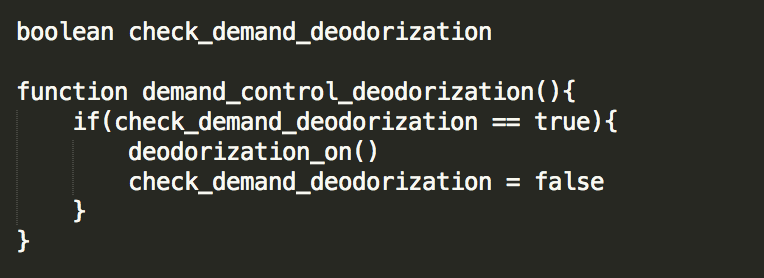
\includegraphics[scale=0.6]{optimization4}
    \label{fig:label}
\end{center}
\end{figure}
\subsubsection{Deodorization function (automatic)}
This function will provide the Smart Shoebox to trigger the deodorant to shoot out in one hour interval. 
%image
\begin{figure}[htbp]
\begin{center}
    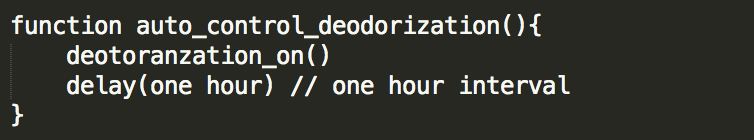
\includegraphics[scale=0.6]{optimization5}
    \label{fig:label}
\end{center}
\end{figure}
\subsubsection{Intensity control feature}
The user can choose the intensity level of fan and lamp. Intensity is calculated as number between 1 to 3, which means maximum, middle, minimum.
%image
\begin{figure}[htbp]
\begin{center}
    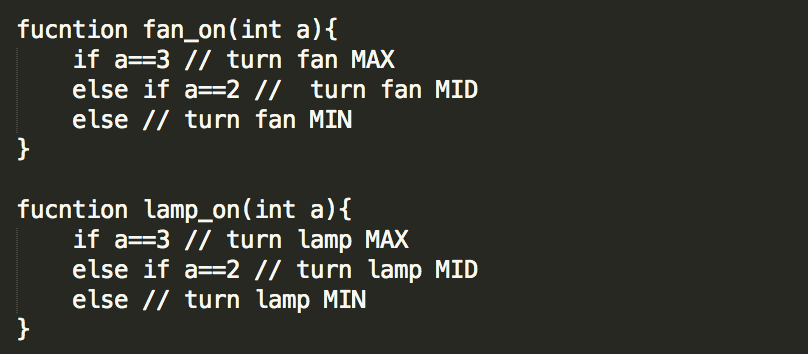
\includegraphics[scale=0.6]{optimization6}
    \label{fig:label}
\end{center}
\end{figure}
\\

\subsection{Management function}
This management function is mostly about modeling and categorizing the shoes. Through the serial number scanning, captured image, 3D scanning and user input, the information about the user and shoes are managed in the database. 
\subsubsection{Shoe categorization function (bar-code scanning)}
\subsubsection{Shoe categorization function (user input based)}
\subsubsection{Shoe categorization function (captured image)}
\subsubsection{Shoe categorization function (3D scanning)}
\subsubsection{Setting the proper management tool}Modeling

The big arrow pointing to the database will be one of the ways of receiving the information of the shoes by the user. Like we mentioned at above part the ways will be the serial number scanning, analyzing the captured image, 3D scanning and analyzing user input.

%image6
\begin{figure}[htbp]
\begin{center}
    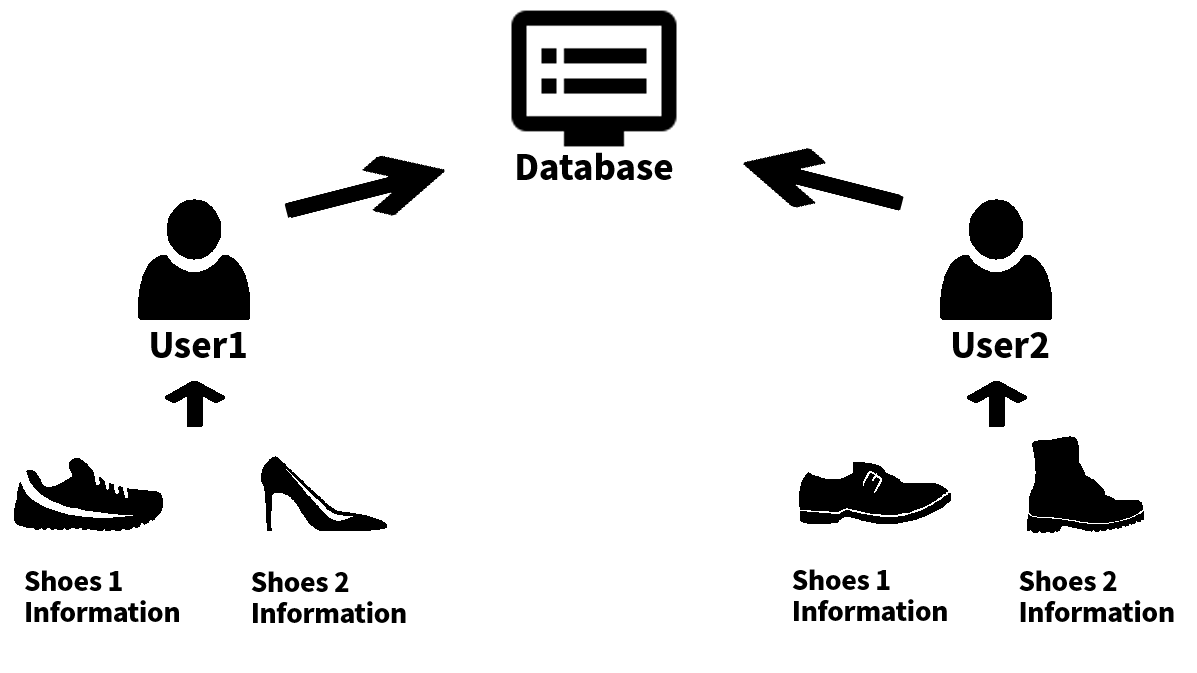
\includegraphics[scale=0.28]{management1}
    \caption{Shoe information into the database} \label{fig:label}
\end{center}
\end{figure}
%image7
\begin{figure}[htbp]
\begin{center}
    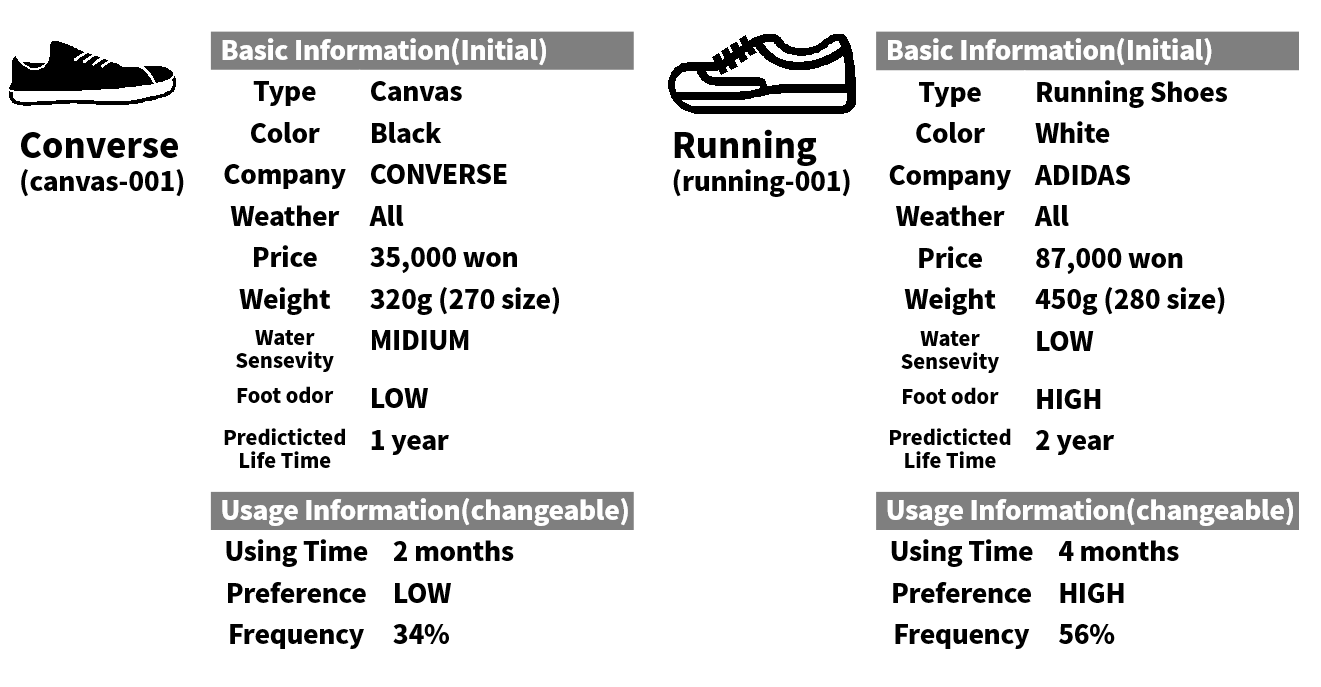
\includegraphics[scale=0.24]{management2}
    \caption{Example of the shoes modeling } \label{fig:label}
\end{center}
\end{figure}

As we can see in Fig.7 the saved information of the shoes will be assigned to each model we will provide before. For each model the proper care solution will be provided. 
The modeling of each shoe into a number of category and setting the proper care solution will be the most important part to realize this function. Also at the same time it is the most ambiguous part before the design phase.



\subsection{Analysis function}
\subsubsection{Absence of shoes analysis (Base information)}
We have decided to analyze the absence of shoes by weight sensor and use it as a base information for other analysis functions. The absence timer will be on and count the time of the shoes absence.
%image
\begin{figure}[htbp]
\begin{center}
    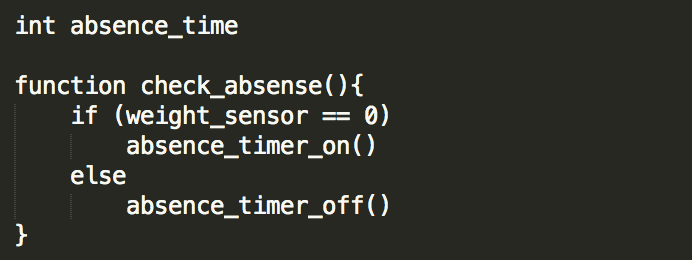
\includegraphics[scale=0.6]{analysis1}
    \label{fig:label}
\end{center}
\end{figure}
\subsubsection{Durability analysis}
Durability is set to decrease by the time the shoe has been put on increases. We have decided the average shoes usage time as 12 hours a day and the durability changes while the absence time increases. Less than 2 weeks is considered to be a new one. Between 2 weeks and 4 weeks is considered to be not bad. 
Between 4 weeks and 8 weeks is considered to be washed. Between 8 weeks and 16 weeks is considered to be careful. More than 16 weeks the shoes is considered to be replaced.
%image
\begin{figure}[htbp]
\begin{center}
    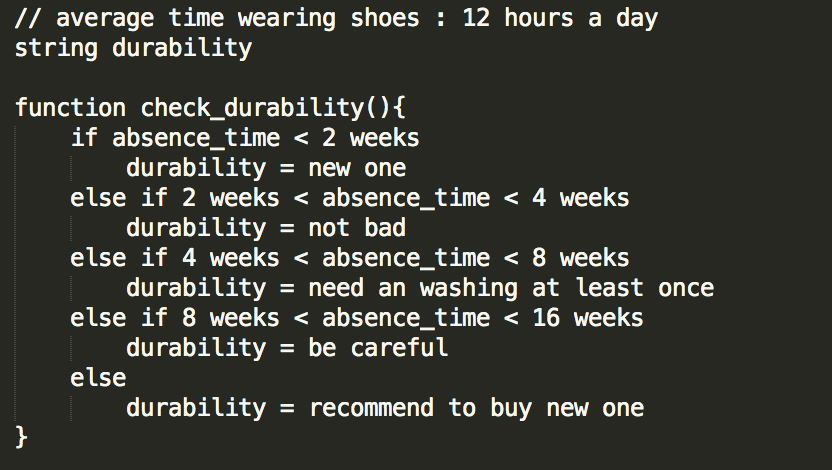
\includegraphics[scale=0.58]{analysis2}
    \label{fig:label}
\end{center}
\end{figure}
\subsubsection{Life prediction analysis}
Based on the information of absence time, we provide the expected  life of the shoes. We subtract the absence time from the original life time.
%image
\begin{figure}[htbp]
\begin{center}
    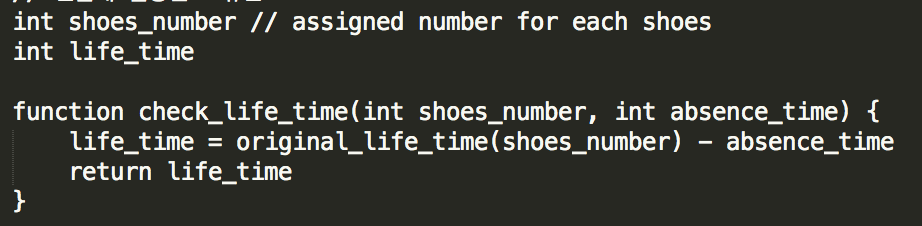
\includegraphics[scale=0.5]{analysis3}
    \label{fig:label}
\end{center}
\end{figure}
\subsubsection{Preference analysis (personal)}
\subsubsection{Preference analysis (general)}
Based on the information of absence time for a number of users, we provide the preference information of the shoes in general aspect. Since we all store the information about the shoes of the user in the database this is possible in both personal and general aspect. Using this Big data, the user can know which shoes are popular nowadays.
%image
\begin{figure}[htbp]
\begin{center}
    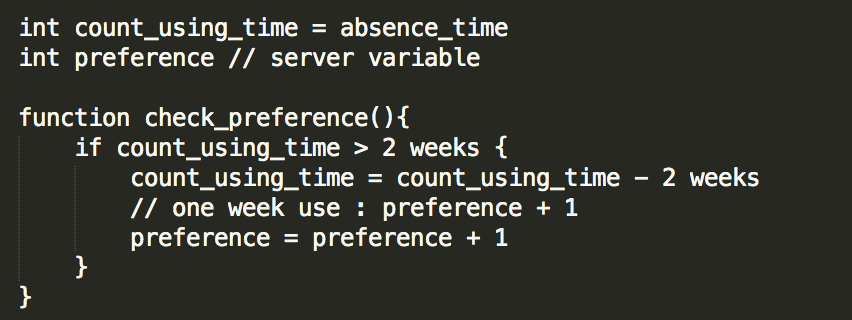
\includegraphics[scale=0.54]{analysis4}
    \label{fig:label}
\end{center}
\end{figure}
\subsubsection{Frequency analysis}
Based on the information of absence time, we provide the frequency information for the shoes in percentage. We devide the used days by the whole day since the user started to use the Smart Shoebox.
%image
\begin{figure}[htbp]
\begin{center}
    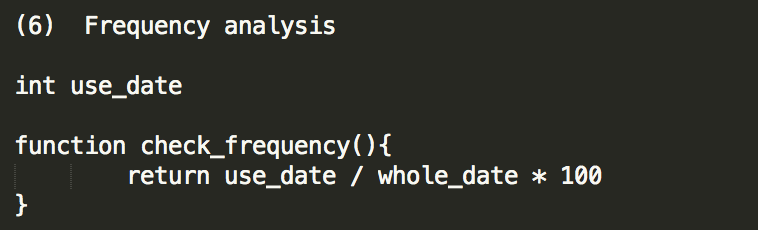
\includegraphics[scale=0.56]{analysis5}
    \label{fig:label}
\end{center}
\end{figure}



\subsection{Recommendation function}
Smart Shoes cabinet will provide recommendation information with percentages based on different kind of aspects. Of course the final choice is up to the user. The main recommendation standard is the weather. So we have decided to place a screen for the weather.
%image8
\begin{figure}[htbp]
\begin{center}
    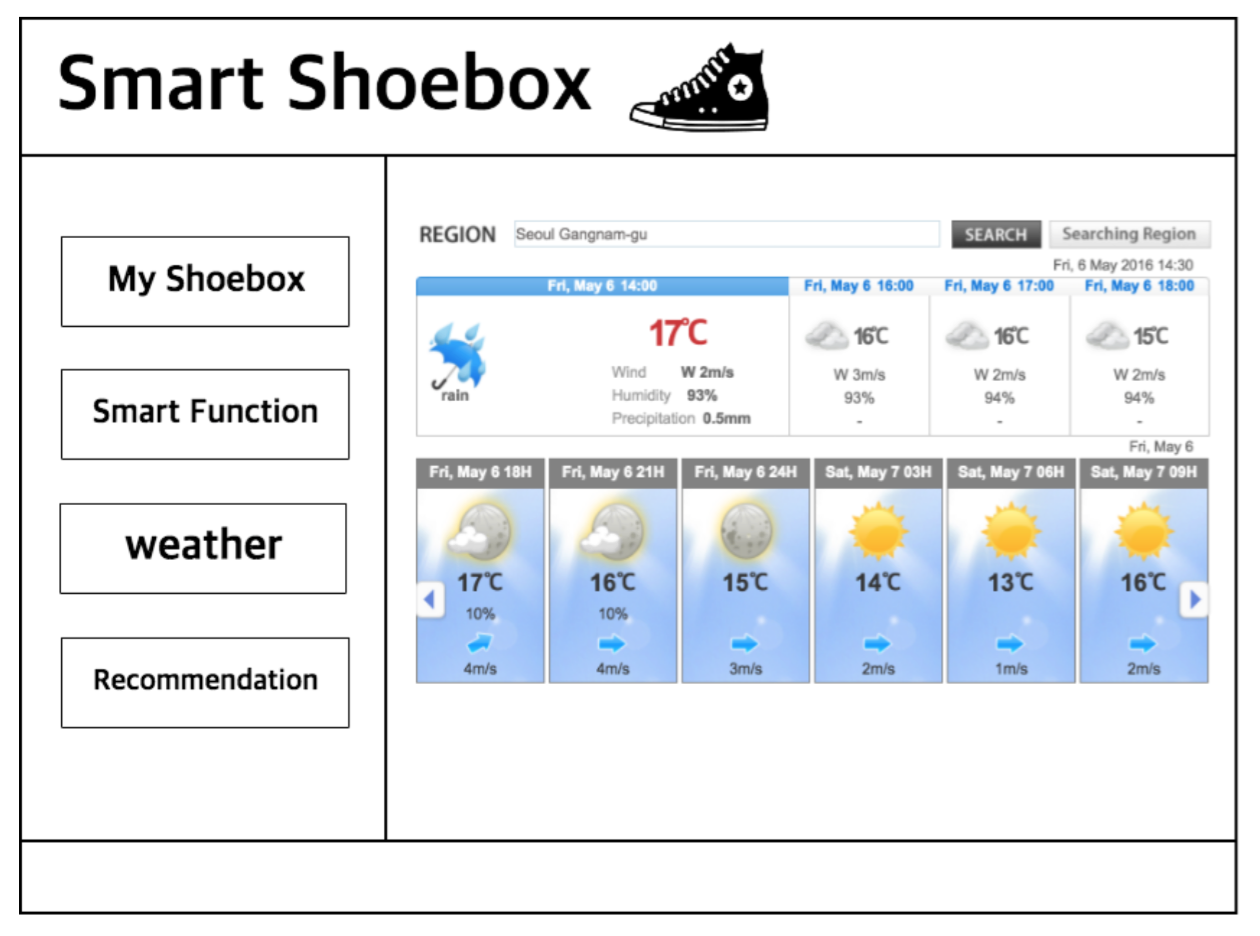
\includegraphics[scale=0.4]{UI1}
   \caption{Weather on the web screen}\label{fig:label}
\end{center}
\end{figure}
%image9
\begin{figure}[htbp]
\begin{center}
    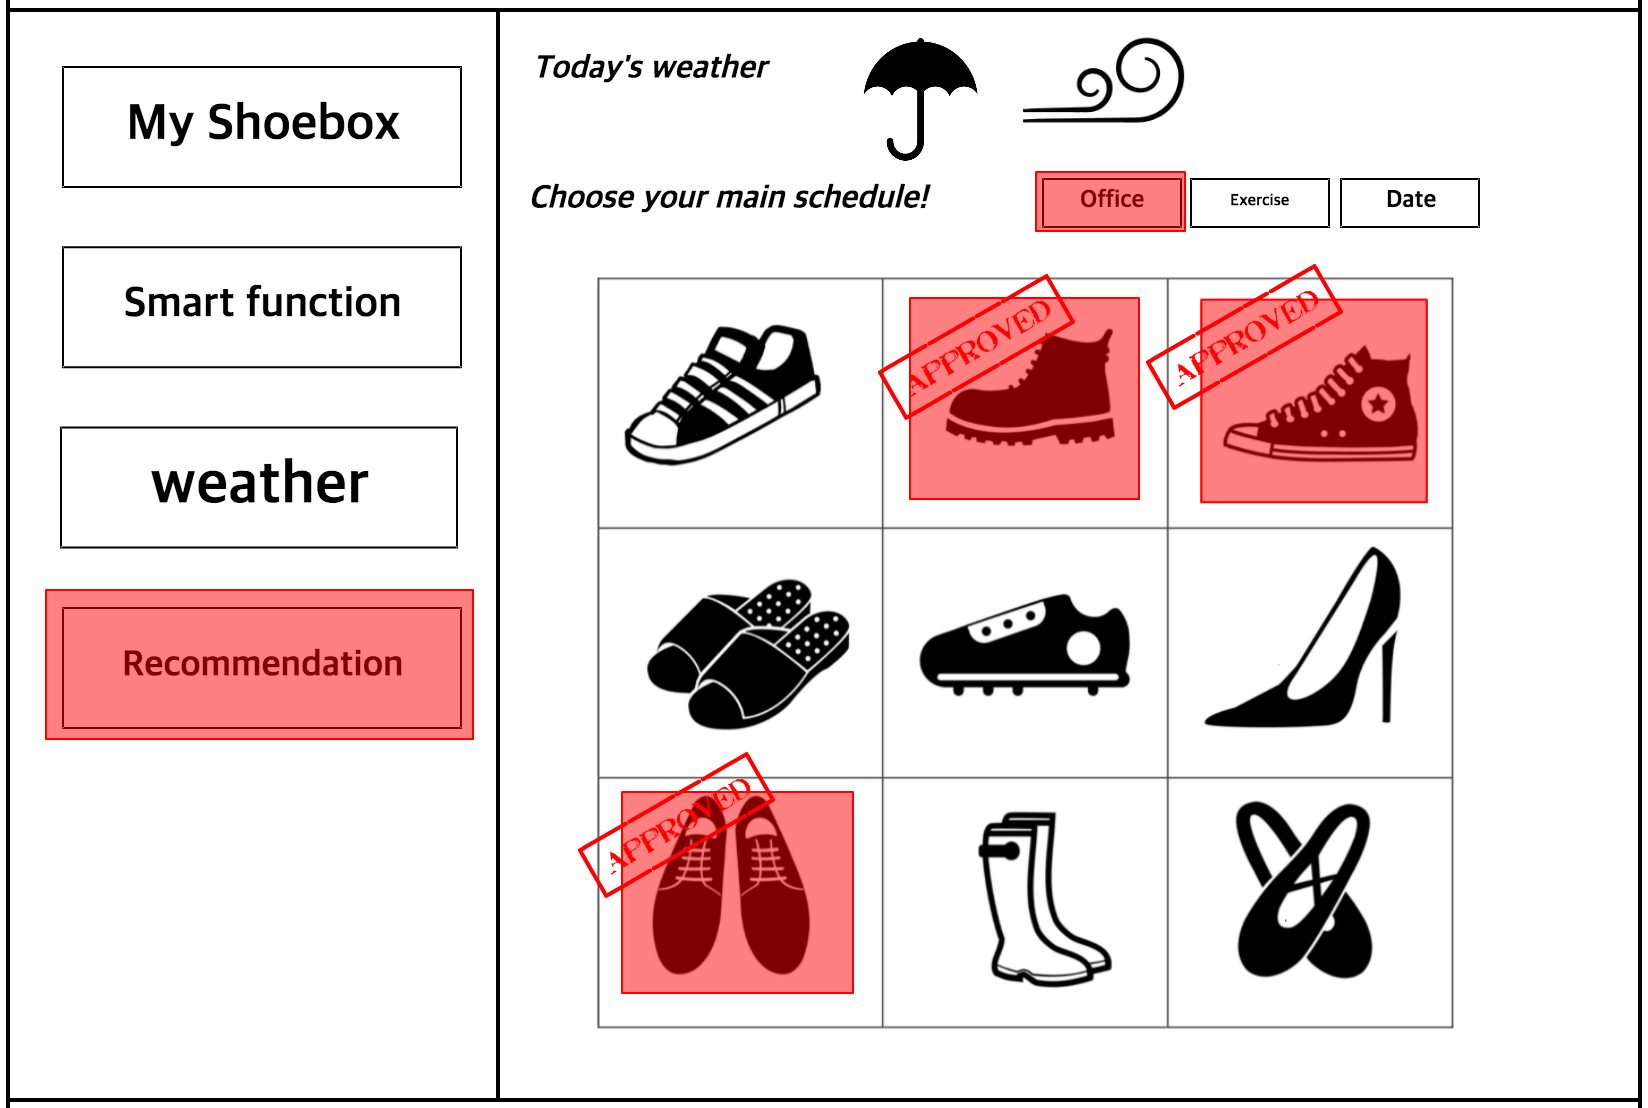
\includegraphics[scale=0.32]{UI2}
   \caption{Recommendation on the web screen}\label{fig:label}
\end{center}
\end{figure}
\subsubsection{Recommendation based on weather forecast }
With weather API, the proper type of shoes is recommended. We decided to classify weather in three cases. ('Sunny' and 'Cloudy' and 'Rainy or Snowy') We will restrict the recommendation choices by the weather becomes bad. The word proper (the proper shoes for the weather) will be represented in the shoes modeled information in the database.
%image
\begin{figure}[htbp]
\begin{center}
    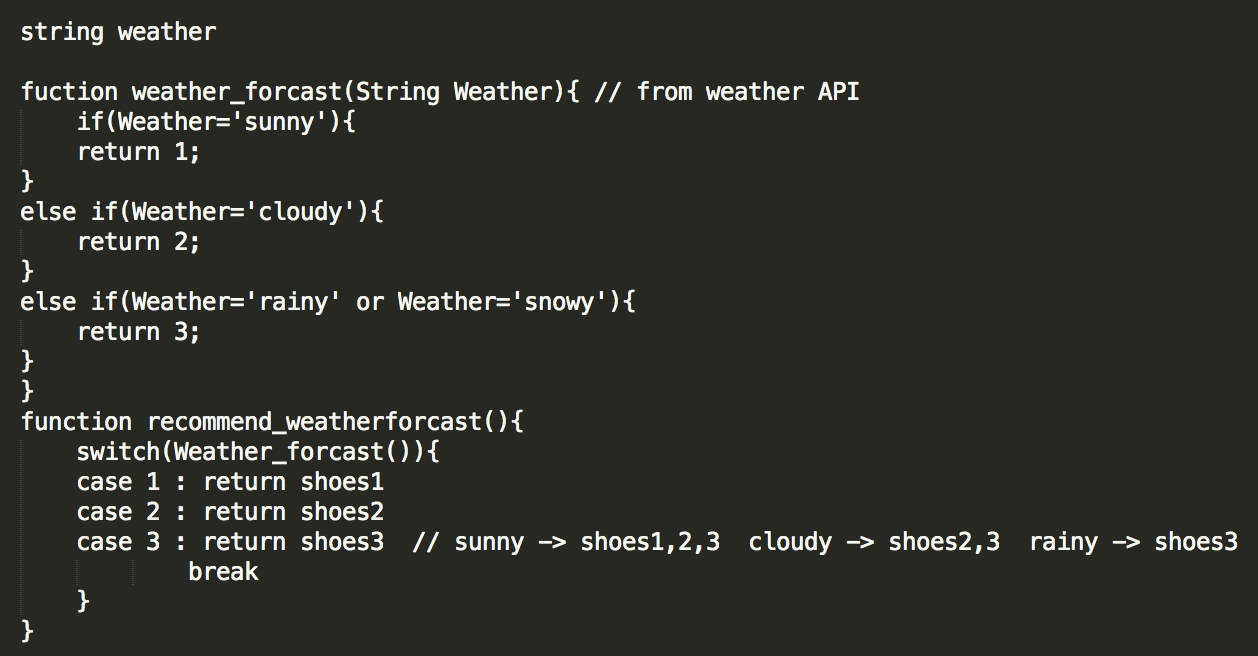
\includegraphics[scale=0.4]{recommendation1}
    \label{fig:label}
\end{center}
\end{figure}
\subsubsection{ Recommendation based on the use of shoes}
Recommending the proper shoes type which matches with the user?s activity. The word proper (the proper shoes for the activity of the user) will be represented in the shoes modeled information in the database.
%image
\begin{figure}[htbp]
\begin{center}
    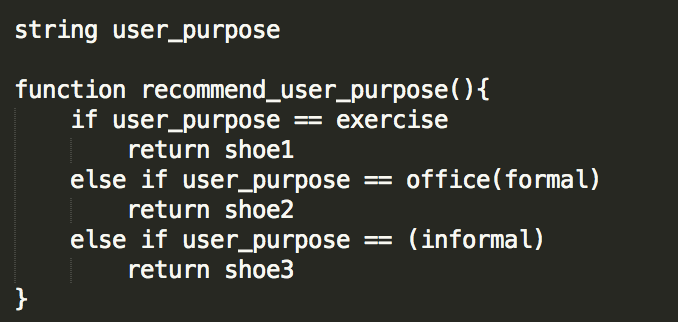
\includegraphics[scale=0.5]{recommendation2}
    \label{fig:label}
\end{center}
\end{figure}
\subsubsection{Recommendation based on the color of shoes}
Recommending the proper shoes color which balances with the users clothing color. The word proper (the proper shoes for the clothes of the user) will be represented in the shoes modeled information in the database.
%image
\begin{figure}[htbp]
\begin{center}
    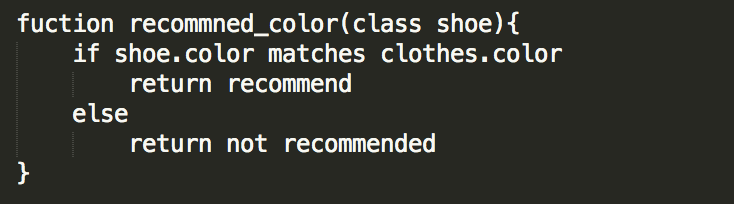
\includegraphics[scale=0.56]{recommendation3}
    \label{fig:label}
\end{center}
\end{figure}
\subsubsection{ Notice of recommendation rate by color}
\subsubsection{Notice of recommendation rate by percentage}
Showing the recommendation rate by different colors. For example, if the shoes are recommended, a specific color will appear on the shoe rack or on the screen the user is looking at. 
Showing the recommendation rate by percentage. If the shoes are recommended strongly, the percentage will appear on the shoe rack or on the screen the user is looking at. 
%image
\begin{figure}[htbp]
\begin{center}
    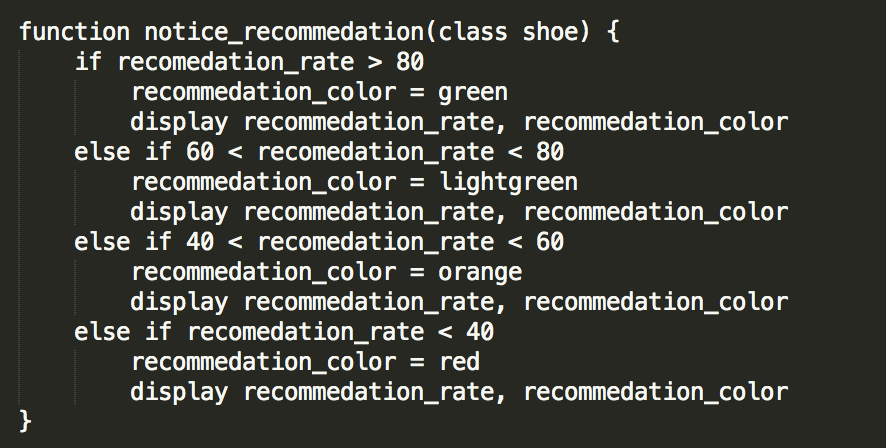
\includegraphics[scale=0.5]{recommendation4}
    \label{fig:label}
\end{center}
\end{figure}


\subsection{Notification function}
\subsubsection{Recognition of contamination by sensor}
\subsubsection{Notification for contamination by message}
With the increased weight, notification is given for contamination. The weight to be sensed is defined to be 20g.
After the recognition of contamination, the information is notified to the user through messages on the screen.
%image
\begin{figure}[htbp]
\begin{center}
    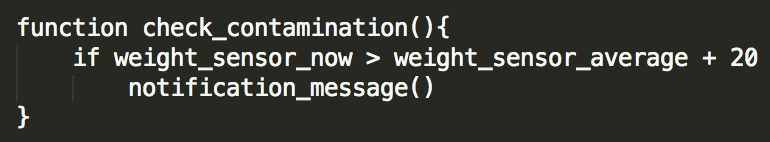
\includegraphics[scale=0.6]{notification1}
    \label{fig:label}
\end{center}
\end{figure}

\subsection{Networking / Remote control function (UI)}
\subsubsection{Control function through web programming (main)}
\subsubsection{Control function through mobile (sub)}
\subsubsection{Control function through embedded system (sub)}
To realize this function we will provide a user interface through mainly web and additionally mobile and a screen for the Smart Shoebox. The already mentioned functions before will be on the UI so that the user can interact with the system. The temperature and humidity will be provided on the screen the user will be seeing. Optimaization function, management function, analysis function, recommendation function, notification function will be on the main screen for users be able to use. 
%image9
\begin{figure}[htbp]
\begin{center}
    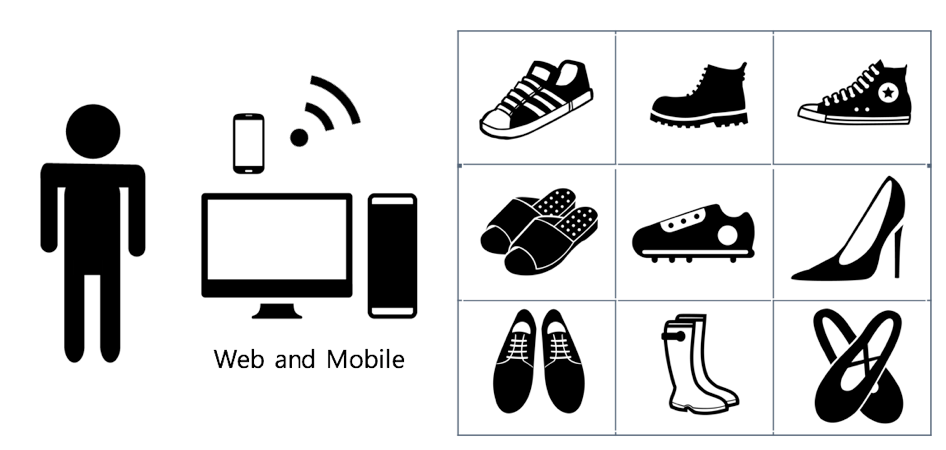
\includegraphics[scale=0.4]{UI3}
   \caption{Networking function through mobile and web}\label{fig:label}
\end{center}
\end{figure}
%image10
\begin{figure}[htbp]
\begin{center}
    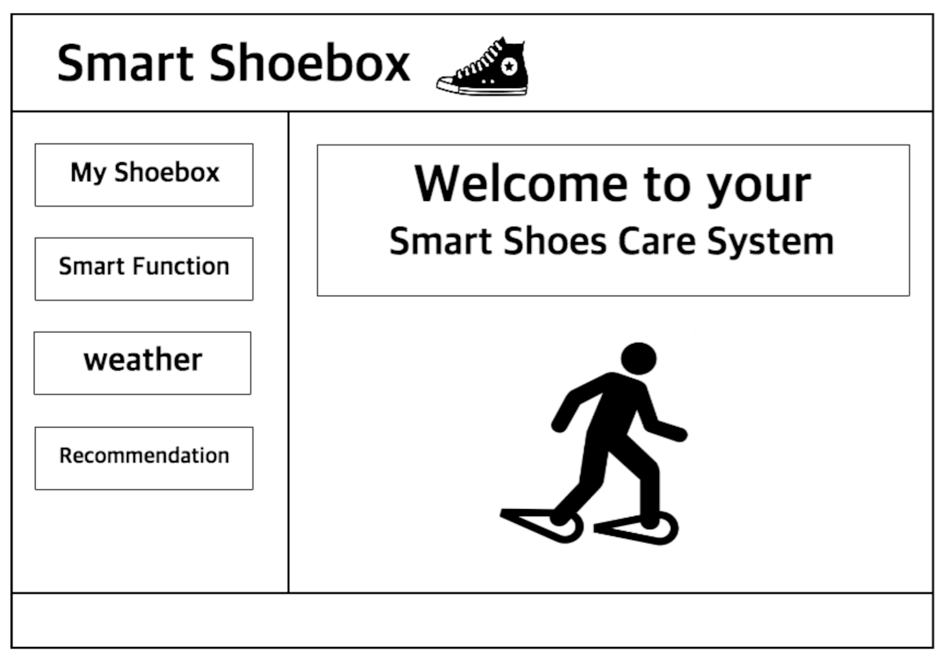
\includegraphics[scale=0.4]{UI4}
   \caption{Main page for Smart Shoebox}\label{fig:label}
\end{center}
\end{figure}
%image11
\begin{figure}[htbp]
\begin{center}
    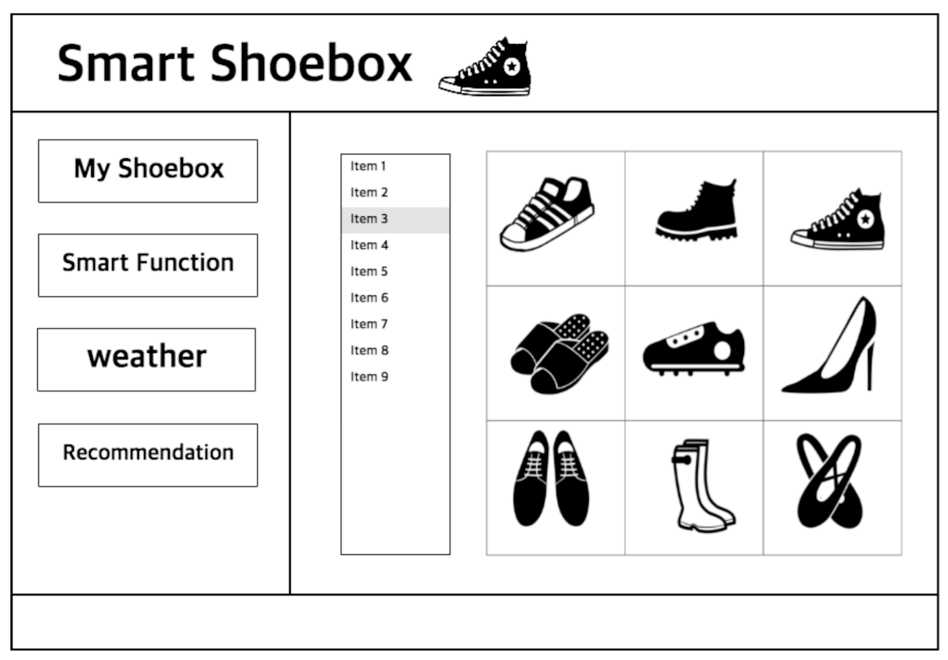
\includegraphics[scale=0.4]{UI5}
   \caption{Shoes status for Smart Shoebox}\label{fig:label}
\end{center}
\end{figure}

% 5. Architecture Design and Implementation
\section{Architecture Design and Implementation}
% 6. use cases
\section{Use Cases}






% An example of a floating figure using the graphicx package.
% Note that \label must occur AFTER (or within) \caption.
% For figures, \caption should occur after the \includegraphics.
% Note that IEEEtran v1.7 and later has special internal code that
% is designed to preserve the operation of \label within \caption
% even when the captionsoff option is in effect. However, because
% of issues like this, it may be the safest practice to put all your
% \label just after \caption rather than within \caption{}.
%
% Reminder: the "draftcls" or "draftclsnofoot", not "draft", class
% option should be used if it is desired that the figures are to be
% displayed while in draft mode.
%
%\begin{figure}[!t]
%\centering
%\includegraphics[width=2.5in]{myfigure}
% where an .eps filename suffix will be assumed under latex, 
% and a .pdf suffix will be assumed for pdflatex; or what has been declared
% via \DeclareGraphicsExtensions.
%\caption{Simulation results for the network.}
%\label{fig_sim}
%\end{figure}

% Note that the IEEE typically puts floats only at the top, even when this
% results in a large percentage of a column being occupied by floats.


% An example of a double column floating figure using two subfigures.
% (The subfig.sty package must be loaded for this to work.)
% The subfigure \label commands are set within each subfloat command,
% and the \label for the overall figure must come after \caption.
% \hfil is used as a separator to get equal spacing.
% Watch out that the combined width of all the subfigures on a 
% line do not exceed the text width or a line break will occur.
%
%\begin{figure*}[!t]
%\centering
%\subfloat[Case I]{\includegraphics[width=2.5in]{box}%
%\label{fig_first_case}}
%\hfil
%\subfloat[Case II]{\includegraphics[width=2.5in]{box}%
%\label{fig_second_case}}
%\caption{Simulation results for the network.}
%\label{fig_sim}
%\end{figure*}
%
% Note that often IEEE papers with subfigures do not employ subfigure
% captions (using the optional argument to \subfloat[]), but instead will
% reference/describe all of them (a), (b), etc., within the main caption.
% Be aware that for subfig.sty to generate the (a), (b), etc., subfigure
% labels, the optional argument to \subfloat must be present. If a
% subcaption is not desired, just leave its contents blank,
% e.g., \subfloat[].


% An example of a floating table. Note that, for IEEE style tables, the
% \caption command should come BEFORE the table and, given that table
% captions serve much like titles, are usually capitalized except for words
% such as a, an, and, as, at, but, by, for, in, nor, of, on, or, the, to
% and up, which are usually not capitalized unless they are the first or
% last word of the caption. Table text will default to \footnotesize as
% the IEEE normally uses this smaller font for tables.
% The \label must come after \caption as always.
%
%\begin{table}[!t]
%% increase table row spacing, adjust to taste
%\renewcommand{\arraystretch}{1.3}
% if using array.sty, it might be a good idea to tweak the value of
%\extrarowheight as needed to properly center the text within the cells
%\caption{An Example of a Table}
%\label{table_example}
%\centering
%% Some packages, such as MDW tools, offer better commands for making tables
%% than the plain LaTeX2e tabular which is used here.
%\begin{tabular}{|c||c|}
%\hline
%One & Two\\
%\hline
%Three & Four\\
%\hline
%\end{tabular}
%\end{table}


% Note that the IEEE does not put floats in the very first column
% - or typically anywhere on the first page for that matter. Also,
% in-text middle ("here") positioning is typically not used, but it
% is allowed and encouraged for Computer Society conferences (but
% not Computer Society journals). Most IEEE journals/conferences use
% top floats exclusively. 
% Note that, LaTeX2e, unlike IEEE journals/conferences, places
% footnotes above bottom floats. This can be corrected via the
% \fnbelowfloat command of the stfloats package.




%\section{Conclusion}
%The conclusion goes here.




% conference papers do not normally have an appendix


% use section* for acknowledgment
%\section*{Acknowledgment}


%The authors would like to thank...





% trigger a \newpage just before the given reference
% number - used to balance the columns on the last page
% adjust value as needed - may need to be readjusted if
% the document is modified later
%\IEEEtriggeratref{8}
% The "triggered" command can be changed if desired:
%\IEEEtriggercmd{\enlargethispage{-5in}}

% references section

% can use a bibliography generated by BibTeX as a .bbl file
% BibTeX documentation can be easily obtained at:
% http://mirror.ctan.org/biblio/bibtex/contrib/doc/
% The IEEEtran BibTeX style support page is at:
% http://www.michaelshell.org/tex/ieeetran/bibtex/
%\bibliographystyle{IEEEtran}
% argument is your BibTeX string definitions and bibliography database(s)
%\bibliography{IEEEabrv,../bib/paper}
%
% <OR> manually copy in the resultant .bbl file
% set second argument of \begin to the number of references
% (used to reserve space for the reference number labels box)
\begin{thebibliography}{1}

\bibitem{IEEEhowto:kopka}
H.~Kopka and P.~W. Daly, \emph{A Guide to \LaTeX}, 3rd~ed.\hskip 1em plus
  0.5em minus 0.4em\relax Harlow, England: Addison-Wesley, 1999.

\end{thebibliography}




% that's all folks
\end{document}